\documentclass[12pt, a4paper]{article}
\usepackage[utf8]{inputenc}
\usepackage{polski}
\usepackage[polish]{babel}
\usepackage{graphicx}
\usepackage{hyperref}
\usepackage[margin=2.5cm]{geometry}
\usepackage{listings}
\usepackage{xcolor}
\usepackage{amsmath}
\usepackage{enumitem}
\usepackage{tikz}
\usepackage{float}
\usepackage{titlesec}
\usepackage[T1]{fontenc}
\usepackage{longtable}
\usepackage{array}
\usepackage{tabularx}
\usepackage{booktabs}
\usepackage{listings}
\usepackage{xcolor}
\usepackage{needspace}
\usepackage{caption}

\lstdefinelanguage{json}{ basicstyle=\ttfamily\small, breaklines=true,
showstringspaces=false, frame=single, morestring=[b]" }

\titleclass{\subsubsubsection}{straight}[
\subsubsection{]}
\newcounter{subsubsubsection}[subsubsection]
\renewcommand{\thesubsubsubsection}{\thesubsubsection.\arabic{subsubsubsection}}
\titleformat{\subsubsubsection}
{\normalfont\normalsize\bfseries}{\thesubsubsubsection}{1em}{}
\titlespacing*{\subsubsubsection}{0pt}{3.25ex plus 1ex minus .2ex}{1.5ex plus .2ex}

\setcounter{tocdepth}{4}

\definecolor{codegreen}{rgb}{0,0.6,0}
\definecolor{codegray}{rgb}{0.5,0.5,0.5}
\definecolor{codepurple}{rgb}{0.58,0,0.82}
\definecolor{backcolour}{rgb}{0.95,0.95,0.95}

\lstdefinestyle{mystyle}{ backgroundcolor=
\color{backcolour}
, commentstyle=
\color{codegreen}
, keywordstyle=
\color{blue}
, stringstyle=
\color{codepurple}
, basicstyle=\ttfamily\scriptsize, breakatwhitespace=false, breaklines=true, captionpos=b,
keepspaces=true, numbersep=5pt, showspaces=false, showstringspaces=false,
showtabs=false, tabsize=2, inputencoding=utf8, extendedchars=true, literate={ą}{{\k{a}}}1
{ć}{{\'c}}1 {ę}{{\k{e}}}1 {ł}{{\l{}}}1 {ń}{{\'n}}1 {ó}{{\'o}}1 {ś}{{\'s}}1 {ż}{{\.z}}1
{ź}{{\'z}}1 {Ą}{{\k{A}}}1 {Ć}{{\'C}}1 {Ę}{{\k{E}}}1 {Ł}{{\L{}}}1 {Ń}{{\'N}}1 {Ó}{{\'O}}1
{Ś}{{\'S}}1 {Ż}{{\.Z}}1 {Ź}{{\'Z}}1 }

\lstset{style=mystyle}

\begin{document}
  \begin{titlepage}
    \begin{center}
      \large {\noindent Collegium Witelona Uczelnia Państwowa w Legnicy}\\
      {\noindent Wydział Nauk Technicznych i Ekonomicznych}\\ {\noindent Kierunek: Informatyka}\\[2cm]
      
\includegraphics[width=5cm]{godlo.jpg}
      \\[2cm]
      {\large\textbf{Podstawy symulacji komputerowej"}}\\[0.3cm]

      {\noindent Temat: ”Opracowanie zadań projektowych”.}\\[2cm] {\large\textbf{Autorzy}}\\
      Mateusz Bogacz-Drewniak, nr. indeksu: 44491\\
      Robert Kuźba, nr. indeksu: 38575\\[2.5cm]	
    \end{center}

    \begin{flushright}
      \begin{tabular}{l}
        Prowadzący przedmiot     \\
        dr inż. Ryszard Rębowski
      \end{tabular}
    \end{flushright}

    \vfill
    \begin{center}
      {\noindent Legnica, 2026}
    \end{center}
  \end{titlepage}

  \tableofcontents
  \newpage
\section{Lista 0 -- zadanie 2}
\subsection{Treść zadania}
Wiadomo, że dla zmiennej losowej $X$ mamy:
\[ X(\Omega)=\{1,2,3,4\} \]
\[ P(\{\omega\in\Omega:X(\omega)=i\})=ic, \quad \text{dla pewnej } c\in \mathbb{R}. \]
Obliczyć dwoma metodami $P(\{\omega\in\Omega:2\le X(\omega)\le3\})$.

\subsection{Rozwiązanie analityczne}

Z własności rozkładu prawdopodobieństwa (warunek unormowania) wiemy, że suma prawdopodobieństw wszystkich zdarzeń elementarnych musi wynosić $1$. Zatem:
\[ \sum_{i=1}^{4} P(X=i) = 1 \]
\[ 1c + 2c + 3c + 4c = 1 \]
\[ 10c = 1 \implies c = \frac{1}{10}. \]

Mając stałą $c$, rozkład zmiennej losowej $X$ prezentuje się następująco:
$P(X=1)=0{,}1$, $P(X=2)=0{,}2$, $P(X=3)=0{,}3$, $P(X=4)=0{,}4$.

\subsubsection{Metoda 1: Bezpośrednie sumowanie prawdopodobieństw} \\
Z racji, że interesują nas zdarzenia dla $X=2$ oraz $X=3$, dodajemy bezpośrednio ich prawdopodobieństwa z wyznaczonego rozkładu:
\[ P(2 \le X \le 3) = P(X=2) + P(X=3) = 0{,}2 + 0{,}3 = 0{,}5. \]

\subsubsection{Metoda 2: Sumowanie z definicji podanej w zadaniu} \\
Wykorzystujemy podany wzór $P(X=i) = i \cdot c$:
\[ P(2 \le X \le 3) = \sum_{i=2}^{3} i \cdot c = 2c + 3c = 5c. \]
Podstawiając $c = \frac{1}{10}$, otrzymujemy:
\[ 5 \cdot \frac{1}{10} = \frac{5}{10} = 0{,}5. \]

\newpage

\subsection{Implementacja}{%
Poniżej przedstawiono kod w języku Python symulujący rozwiązanie tego zadania wraz z generacją wykresów rozkładu zmiennej losowej i jej dystrybuanty.
}

\Needspace{22\baselineskip}
\begin{lstlisting}[language=Python, caption=Implementacja dwóch rozwiążań zadania]
import matplotlib.pyplot as plt
import numpy as np

print("\n1.Znalezienie stalej c:")
print("X(Ω) = {1, 2, 3, 4}")
print("P(X = i) = i·c")
print("\nWarunek: suma wszystkich prawdopodobienstw = 1")
print("P(X=1) + P(X=2) + P(X=3) + P(X=4) = 1")
print("1·c + 2·c + 3·c + 4·c = 1")
print("10·c = 1\n")

c = 1/10
print(f"\033[1mStala c:\033[0m {c} \n")
values = [1, 2, 3, 4]
probabilities = [i * c for i in values]

print(f"P(X=1) = 1·{c} = {probabilities[0]}")
print(f"P(X=2) = 2·{c} = {probabilities[1]}")
print(f"P(X=3) = 3·{c} = {probabilities[2]}")
print(f"P(X=4) = 4·{c} = {probabilities[3]} \n")
print(f"\033[1mSuma:\033[0m {sum(probabilities)} \n")

print("Metoda 1: Bezposrednie sumowanie")
print("P(2 ≤ X ≤ 3) = P(X=2) + P(X=3)")
print(f"= 2·c + 3·c")
print(f"= 2·{c} + 3·{c}")
print(f"= {2*c} + {3*c}")

result_method1 = probabilities[1] + probabilities[2]
print(f"\033[1m= {result_method1} \033[0m\n")

print("Metoda 2: Przez sumowanie zdan 2 i 3 z definicji")
print("P(2 ≤ X ≤ 3) = Σ P(X=i) dla i ∈ {2, 3}")

result_method2 = sum(probabilities[i-1] for i in [2, 3])
print(f"= {probabilities[1]} + {probabilities[2]}")

print(f"\033[1m= {result_method2} \033[0m\n")

print("Weryfikacaja zgodnosci wynikow:")
print(f"\033[1mMetoda 1: {result_method1}\033[0m")
print(f"\033[1mMetoda 2: {result_method2}\033[0m")
print(f"\033[1mZgodnosc: {'Tak' if abs(result_method1 - result_method2) < 1e-10 else 'Nie'}\033[0m\n")

fig, axes = plt.subplots(1, 2, figsize=(14, 5))

ax1 = axes[0]
colors = ['lightblue', 'salmon', 'salmon', 'lightblue']
bars = ax1.bar(values, probabilities, color=colors, edgecolor='black', linewidth=2, width=0.6)

bars[1].set_color('salmon')
bars[2].set_color('salmon')

ax1.set_xlabel('X', fontsize=12, fontweight='bold')
ax1.set_ylabel('P(X = i)', fontsize=12, fontweight='bold')
ax1.set_title('Rozklad zmiennej losowej X', fontsize=13, fontweight='bold')
ax1.set_xticks(values)
ax1.grid(axis='y', alpha=0.3, linestyle='--')
ax1.set_ylim([0, max(probabilities) * 1.2])

for i, (val, prob) in enumerate(zip(values, probabilities)):
    ax1.text(val, prob + 0.01, f'{prob:.1f}', ha='center', fontsize=11, fontweight='bold')

ax1.text(0.5, 0.95, 'Kolor jasnoniebieski: nie wliczone do P(2 ≤ X ≤ 3)', 
         transform=ax1.transAxes, fontsize=10, verticalalignment='top',
         bbox=dict(boxstyle='round', facecolor='lightblue', alpha=0.5))
ax1.text(0.5, 0.85, 'Kolor lososiowy: wliczone do P(2 ≤ X ≤ 3)', 
         transform=ax1.transAxes, fontsize=10, verticalalignment='top',
         bbox=dict(boxstyle='round', facecolor='salmon', alpha=0.5))

ax2 = axes[1]
cumulative_probs = np.cumsum(probabilities)
x_cdf = [0] + values
y_cdf = [0] + list(cumulative_probs)

ax2.step(x_cdf, y_cdf, 'b-', linewidth=2, marker='o', markersize=8, where='post', label='F(x) = P(X ≤ x)')
ax2.fill_between([1.99, 3.01], 0, 1, alpha=0.3, color='salmon', label='P(2 ≤ X ≤ 3)')

ax2.set_xlabel('X', fontsize=12, fontweight='bold')
ax2.set_ylabel('F(X)', fontsize=12, fontweight='bold')
ax2.set_title('Dystrybuanta zmiennej losowej X', fontsize=13, fontweight='bold')
ax2.grid(True, alpha=0.3, linestyle='--')
ax2.set_xlim([-0.5, 5])
ax2.set_ylim([-0.05, 1.1])
ax2.legend(fontsize=10)

for i, cum_prob in enumerate(cumulative_probs):
    ax2.text(x_cdf[i], cum_prob + 0.05, f'{cum_prob:.2f}', ha='center', fontsize=9)

plt.tight_layout()
print("\nWizualizacja zapisana do: zad2_lista0_visualization.png \n")
plt.show()

print(f"\033[1mPodsumowanie:\033[0m")
print(f"P(2 ≤ X ≤ 3) = {result_method1} = {result_method1.as_integer_ratio()[0]}/{result_method1.as_integer_ratio()[1]} = 50%")
\end{lstlisting}

\subsection{Odpowiedź końcowa}{%
Obydwie metody analityczne, jak i weryfikacja numeryczna za pomocą skryptu Python, doprowadziły do tego samego wyniku. Szukane prawdopodobieństwo wynosi:
}

\Needspace{12\baselineskip}
\[
\boxed{P(2 \le X \le 3) = 0{,}5}
\]

czyli:

\[
\boxed{50\%}.
\]

\newpage

\section{Lista 1 - zadanie 2}
\subsection{Treść zadania}
Napisać program wykonujący algorytm kwadratowy von Neumanna.

\subsection{Opis metody}
Algorytm środka kwadratu (zaproponowany przez Johna von Neumanna) to jedna z najstarszych metod generowania liczb pseudolosowych. Metoda opiera się na następujących krokach:
\begin{enumerate}
    \item Wybór początkowej wartości ziarna (ang. \textit{seed}) o długości $n$ cyfr.
    \item Podniesienie tej wartości do kwadratu, co daje liczbę o długości do $2n$ cyfr.
    \item Uzupełnienie wyniku zerami wiodącymi (jeśli to konieczne), aby zachować stałą długość $2n$.
    \item Wyciągnięcie $n$ środkowych cyfr, które stają się kolejną wygenerowaną liczbą i nowym ziarnem dla następnej iteracji.
\end{enumerate}
Częstym problemem tego algorytmu jest szybkie zapętlanie się lub zbieganie do zera. W poniższej implementacji wprowadzono mechanizm zapobiegający temu zjawisku poprzez resetowanie wartości w przypadku osiągnięcia zera.

\subsection{Implementacja}
Symulację wykonano w języku Python. Poniżej przedstawiono implementację generatora oraz funkcji wizualizujących niezależność wygenerowanych próbek w przestrzeni 2D i 3D:

\begin{lstlisting}[language=Python, caption=Implementacja algorytmu kwadratowego von Neumanna]
import matplotlib.pyplot as plt

def von_neumann_generator(seed, n_samples):
    current = seed
    results = []
    
    for i in range(n_samples):
        # Podniesienie do kwadratu i wyrownanie do 8 znakow
        square_str = str(current**2).zfill(8)
        
        # Pobranie 4 srodkowych cyfr (indeksy 2,3,4,5)
        middle_str = square_str[2:6]
        current = int(middle_str)
        
        # Normalizacja do przedzialu [0, 1)
        results.append(current / 10000.0)
        
        # Zabezpieczenie przed utknieciem w zerze
        if current == 0:
            current = 1234 + i 
            
    return results

def plot_2d_independence(data):
    x = data[:-1]
    y = data[1:]
    
    plt.figure(figsize=(8, 8))
    plt.scatter(x, y, alpha=0.6, s=15, color='blue')
    plt.title("Test graficzny 2D: Von Neumann ($r_n$ vs $r_{n+1}$)")
    plt.xlabel("$r_n$")
    plt.ylabel("$r_{n+1}$")
    plt.grid(True, linestyle='--', alpha=0.5)
    plt.show()

def plot_3d_independence(data):
    # Tworzymy trojki (x, y, z)
    x = data[:-2]
    y = data[1:-1]
    z = data[2:]
    
    fig = plt.figure(figsize=(10, 8))
    ax = fig.add_subplot(111, projection='3d')
    
    ax.scatter(x, y, z, alpha=0.6, s=10, color='purple')
    ax.set_title("Test graficzny 3D: Von Neumann ($r_n, r_{n+1}, r_{n+2}$)")
    ax.set_xlabel("$r_n$")
    ax.set_ylabel("$r_{n+1}$")
    ax.set_zlabel("$r_{n+2}$")
    plt.show()
    
# Wykonanie algorytmu
samples = von_neumann_generator(seed=1234, n_samples=500)
\end{lstlisting}

\subsection{Wyniki symulacji i testy graficzne}
Wygenerowano próbkę $N = 500$ liczb pseudolosowych dla początkowego ziarna $1234$. 
Pierwsze wartości wygenerowanego ciągu to m.in.: $0.5227, 0.3215, 0.0336, 0.1128$.

Aby sprawdzić jakość wygenerowanego ciągu i niezależność kolejnych próbek, przeprowadzono testy graficzne w wymiarze 2D (punkty o współrzędnych $r_n, r_{n+1}$) oraz 3D (punkty o współrzędnych $r_n, r_{n+1}, r_{n+2}$).

\begin{figure}[H]
    \centering
    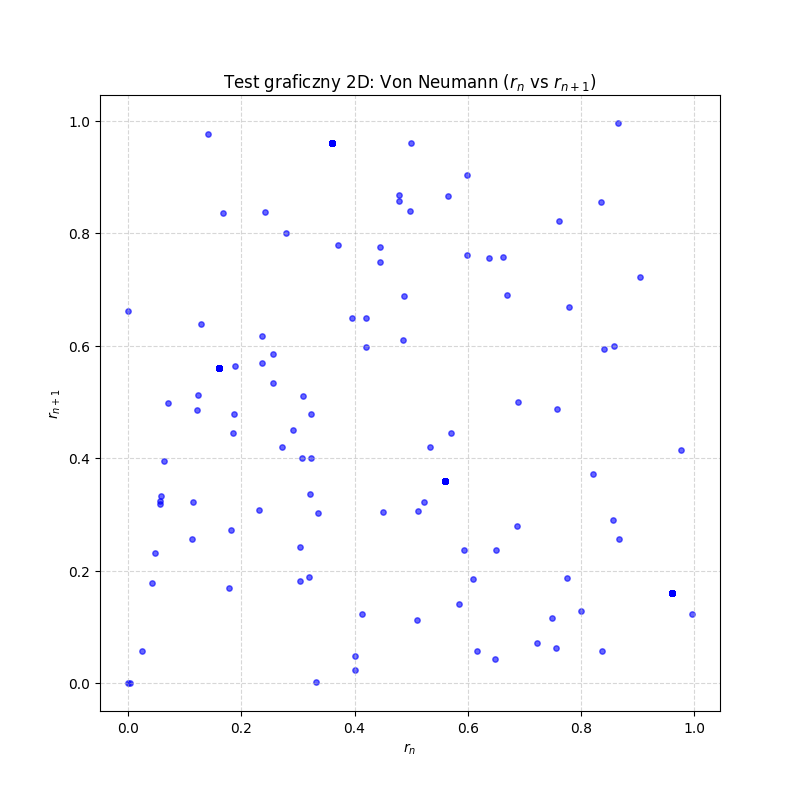
\includegraphics[width=0.8\textwidth]{wykres2d.png}
    \caption{Rozkład par $(r_n, r_{n+1})$ w teście 2D.}
\end{figure}

\begin{figure}[H]
    \centering
    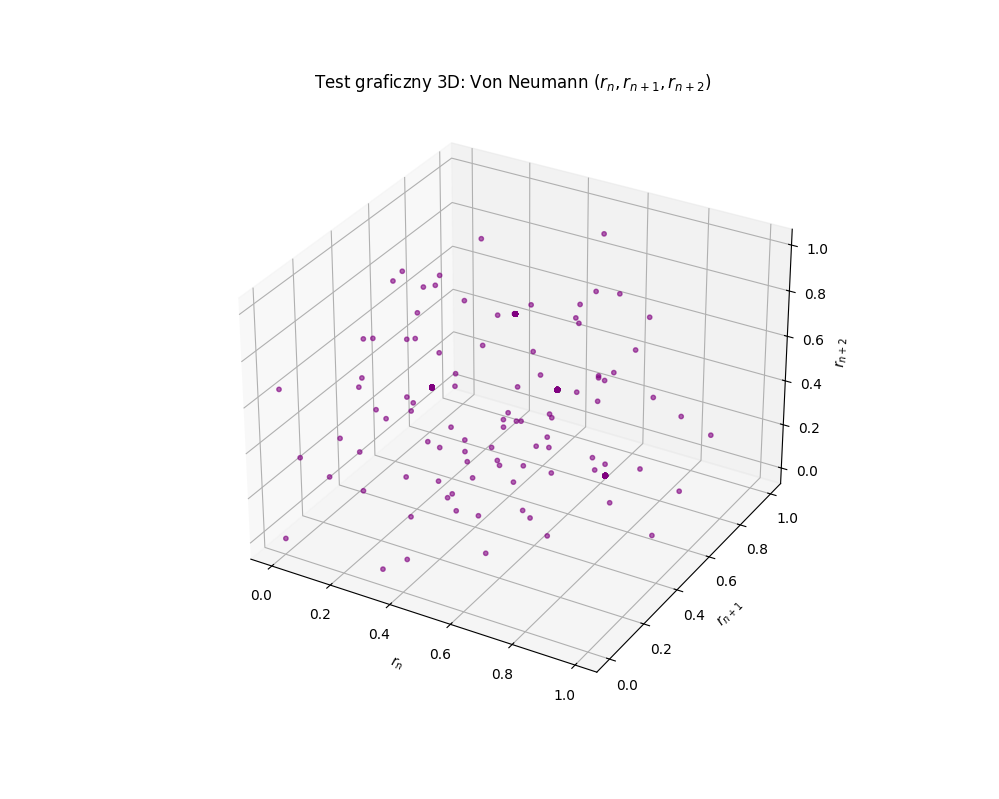
\includegraphics[width=0.8\textwidth]{wykres3d.png}
    \caption{Rozkład trójek $(r_n, r_{n+1}, r_{n+2})$ w teście 3D.}
\end{figure}

\subsection{Interpretacja wyników}
Na podstawie przeprowadzonych testów graficznych (wykresy 2D i 3D) można wstępnie ocenić jakość generatora. Zbyt wyraźne wzory, prążki lub skupiska punktów na wykresach świadczyłyby o silnej zależności między kolejnymi próbkami, co jest charakterystyczną wadą prostych generatorów (takich jak klasyczny algorytm von Neumanna). Zastosowane w kodzie zabezpieczenie (zmiana stanu przy wygenerowaniu $0$) zapobiega całkowitej degradacji ciągu, jednak dla profesjonalnych zastosowań symulacyjnych metoda ta ustępuje nowoczesnym generatorom.

\section{Lista 2 - zadanie 5}
\subsection{Treść zadania }

Zakładamy, że szkody klientów zgłaszane są według procesu Poissona
o intensywności 10 na dzień. Kwota szkody jest zmienną losową o rozkładzie
wykładniczym ze średnią \$1000. Firma ubezpieczeniowa otrzymuje wpłaty
w sposób ciągły ze stałą intensywnością \$11000 na dzień. Przyjmując kapitał
początkowy \$25000, oszacować metodą symulacji prawdopodobieństwo, że kapitał
pozostanie dodatni przez pierwsze 365 dni.

\newpage

\subsection{Model probabilistyczny}
Niech $U(t)$ oznacza kapitał firmy w chwili $t$, gdzie $t\in[0,365]$.
}
Przyjmujemy:
\[
U(0)=25000.
\]

Wpłaty napływają ciągle ze stałą intensywnością:
\[
c=11000 \quad \text{[\$ na dzień]}.
\]

Między kolejnymi szkodami kapitał zmienia się liniowo:
\[
\frac{\mathrm{d}U}{\mathrm{d}t}=c,
\]
o ile nie wystąpi zdarzenie szkody.

Zgłoszenia szkód tworzą proces Poissona o intensywności:
\[
\lambda=10 \quad \text{[zdarzeń na dzień]}.
\]

Oznacza to, że czasy między kolejnymi szkodami są niezależne i mają rozkład
wykładniczy:
\[
T_i \sim \mathrm{Exp}(\lambda),
\]
przy czym średni czas między szkodami wynosi $1/\lambda=0{,}1$ dnia.

Kwota pojedynczej szkody $X_i$ jest zmienną losową o rozkładzie wykładniczym
ze średnią \$1000:
\[
E(X_i)=1000,
\]
czyli parametr skali wynosi $1000$, a gęstość:
\[
f(x)=\frac{1}{1000}e^{-x/1000},\qquad x>0.
\]

W chwili wystąpienia $i$-tej szkody kapitał ulega natychmiastowej redukcji:
\[
U(t_i^+)=U(t_i^-)-X_i.
\]

Szukane jest prawdopodobieństwo:
\[
p=P\big(U(t)>0 \text{ dla wszystkich } t\in[0,365]\big).
\]

\newpage

\subsection{Metoda zdarzeń dyskretnych}
W metodzie zdarzeń dyskretnych symulujemy tylko chwile, w których stan systemu
ulega zmianie. W tym modelu są to wyłącznie chwile zgłoszenia szkód.

Algorytm jednej replikacji:
}

\Needspace{16\baselineskip}
\begin{enumerate}
    \item Ustaw $t=0$ oraz $U=25000$.
    \item Wygeneruj odstęp do kolejnej szkody:
    \[
    \Delta \sim \mathrm{Exp}(\lambda).
    \]
    \item Jeżeli $t+\Delta>365$, dolicz wpłaty do końca roku i zakończ replikację.
    \item W przeciwnym razie:
    \begin{itemize}
        \item zwiększ kapitał o wpłaty w okresie $(t,t+\Delta)$:
        \[
        U \leftarrow U + c\Delta;
        \]
        \item ustaw $t\leftarrow t+\Delta$;
        \item wygeneruj kwotę szkody $X\sim \mathrm{Exp}(1000)$;
        \item zmniejsz kapitał: $U\leftarrow U-X$;
        \item jeżeli $U\le 0$, zakończ replikację wynikiem negatywnym.
    \end{itemize}
    \item Powtarzaj krok 2.
\end{enumerate}

Ponieważ między szkodami kapitał rośnie liniowo, minimum na każdym takim
odcinku występuje bezpośrednio po obsłużeniu szkody. Wystarczy zatem sprawdzać
warunek dodatniego kapitału po każdym zdarzeniu szkody.

\newpage

\subsection{Implementacja}

Symulację wykonano w języku Python. Poniżej przedstawiono główną funkcję
jednej replikacji:
}

\Needspace{22\baselineskip}
\begin{lstlisting}[language=Python, caption=Fragment kodu przedstawiącą replikacje]
def symuluj_jedna_sciezke():
    czas = 0.0
    kapital = 25000.0

    while True:
        odstep = random.expovariate(10.0)
        czas_szkody = czas + odstep

        if czas_szkody > 365.0:
            kapital += 11000.0 * (365.0 - czas)
            return kapital > 0.0

        kapital += 11000.0 * (czas_szkody - czas)
        czas = czas_szkody

        kwota_szkody = random.expovariate(1.0 / 1000.0)
        kapital -= kwota_szkody

        if kapital <= 0.0:
            return False
\end{lstlisting}

Prawdopodobieństwo $p$ estymujemy metodą Monte Carlo:
\[
\hat{p}=\frac{1}{N}\sum_{j=1}^{N} I_j,
\]
gdzie $I_j=1$, jeżeli w $j$-tej replikacji kapitał pozostał dodatni przez cały
okres $[0,365]$, a w przeciwnym razie $I_j=0$.

W obliczeniach przyjęto:
\[
N=100000.
\]

\subsection{Wyniki symulacji}
Po wykonaniu $N=100000$ niezależnych replikacji otrzymano:

\Needspace{10\baselineskip}
\begin{center}
\captionof{table}{Wyniki estymacji parametrów symulacji} % Tutaj wpisz swój tytuł
\[
\begin{array}{l|r}
\text{Wielkość} & \text{Wartość}\\
\hline
\text{Liczba replikacji} & 100000\\
\text{Liczba sukcesów} & 90637\\
\text{Liczba niepowodzeń} & 9363\\
\text{Estymator } \hat{p} & 0{,}9064\\
\text{95\% przedział ufności} & (0{,}9045;\ 0{,}9082)
\end{array}
\]
\end{center}

Oznacza to, że w około $90{,}64\%$ symulowanych scenariuszy kapitał firmy
pozostał dodatni przez cały rok.

\sekcjazwstep{Interpretacja wyniku}{%
Średnia liczba szkód w ciągu 365 dni wynosi około:
}
\[
\lambda \cdot 365 = 10 \cdot 365 = 3650.
\]

Średni łączny koszt szkód:
\[
3650 \cdot 1000 = 3\,650\,000.
\]

Średni napływ wpłat w ciągu roku:
\[
11000 \cdot 365 = 4\,015\,000.
\]

Teoretyczna średnia zmiana kapitału (bez uwzględnienia zmienności) jest dodatnia,
jednak duża losowość kwot pojedynczych szkód powoduje, że w części scenariuszy
następuje bankructwo.

\subsection{Odpowiedź końcowa}
Metodą zdarzeń dyskretnych oszacowano, że prawdopodobieństwo utrzymania dodatniego
kapitału przez pierwsze 365 dni wynosi:

\Needspace{12\baselineskip}
\[
\boxed{\hat{p}\approx 0{,}9064}
\]

czyli około:

\[
\boxed{90{,}6\%}.
\]

Przy $95\%$ poziomie ufności można przyjąć przedział:

\[
\boxed{(0{,}9045;\ 0{,}9082)}.
\]

  \newpage
  \renewcommand{\lstlistlistingname}{Spis fragmentów kodu}

  \listoffigures
  \vspace{1cm}
  \listoftables
  \vspace{1cm}
  \lstlistoflistings
\end{document}